\documentclass{article}
\usepackage{fancyvrb}
\usepackage{a4wide}
\usepackage[T1]{fontenc}
\usepackage[utf8]{inputenc}
\usepackage[french]{babel}
\usepackage{empheq}
\usepackage{mathtools, bm}
\usepackage{amssymb, bm}
\usepackage{graphicx}
\usepackage{caption}
\usepackage{subcaption}
\usepackage{hyperref}
\usepackage{csvsimple}
\usepackage{float}
\usepackage{wrapfig}

\title{\textbf{\Huge  Université Paris Saclay}\\ Prédiction d'arrestations criminelles}
\author{Guillaume Abadie, Jérôme Coquisart, Mathis Dupont, Martin Vitani}
\date{Année 2021}


\begin{document}
    \maketitle
    %\vspace{100px}
    \tableofcontents

    \section{Introduction au problème}
    La ville de Chicago a un ratio de crimes, surtout sur les crimes violents,
    au dessus de la moyenne nationale des États-Unis.
    Les crimes dans la ville ont été collectés dès le début du 20ème siècle pour
    essayer de comprendre pourquoi la ville était sujette à autant de violence.
    Le \href{https://www.kaggle.com/n3v375/chicago-crime-from-01jan2001-to-22jul2020}{dataset} correspond aux crimes commis entre 2001 et 2020, et contient environ 
    7 millions d'entrées.
    Tous les jours, la police de Chicago alimente la base de données avec les
    nouveaux crimes commis dans la ville. 
    Parmi les données collectées, on retrouve: 
    cambriolages, agressions, homicides, vols, braquages, intimidations, kidnapping, 
    possession d'arme\dots.
    Seuls les meurtres ne sont pas comptabilisés dans la base de données.

    \section{Aperçu du dataset}
    \begin{figure}[H]
	    \centering
	    \begin{subfigure}{.45\textwidth}
		    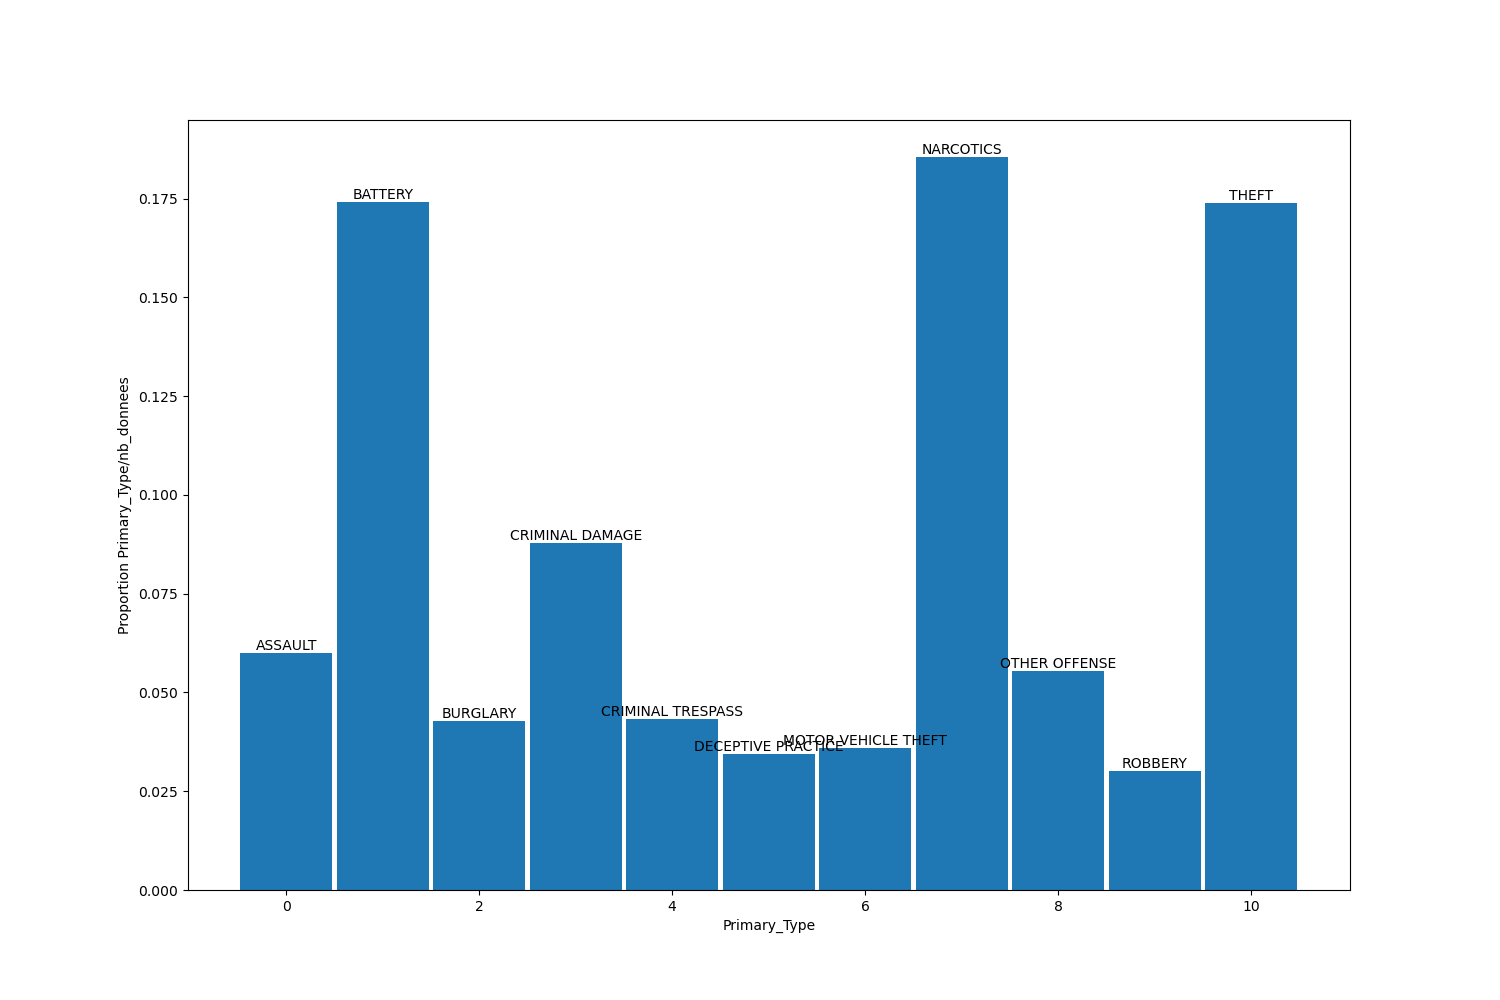
\includegraphics[scale=.2]{images/pprimarytype.png}
		    \caption{Pourcentage de crimes en fonction de leurs type}
		    \label{A}
	    \end{subfigure}
	    \begin{subfigure}{.45\textwidth}
		    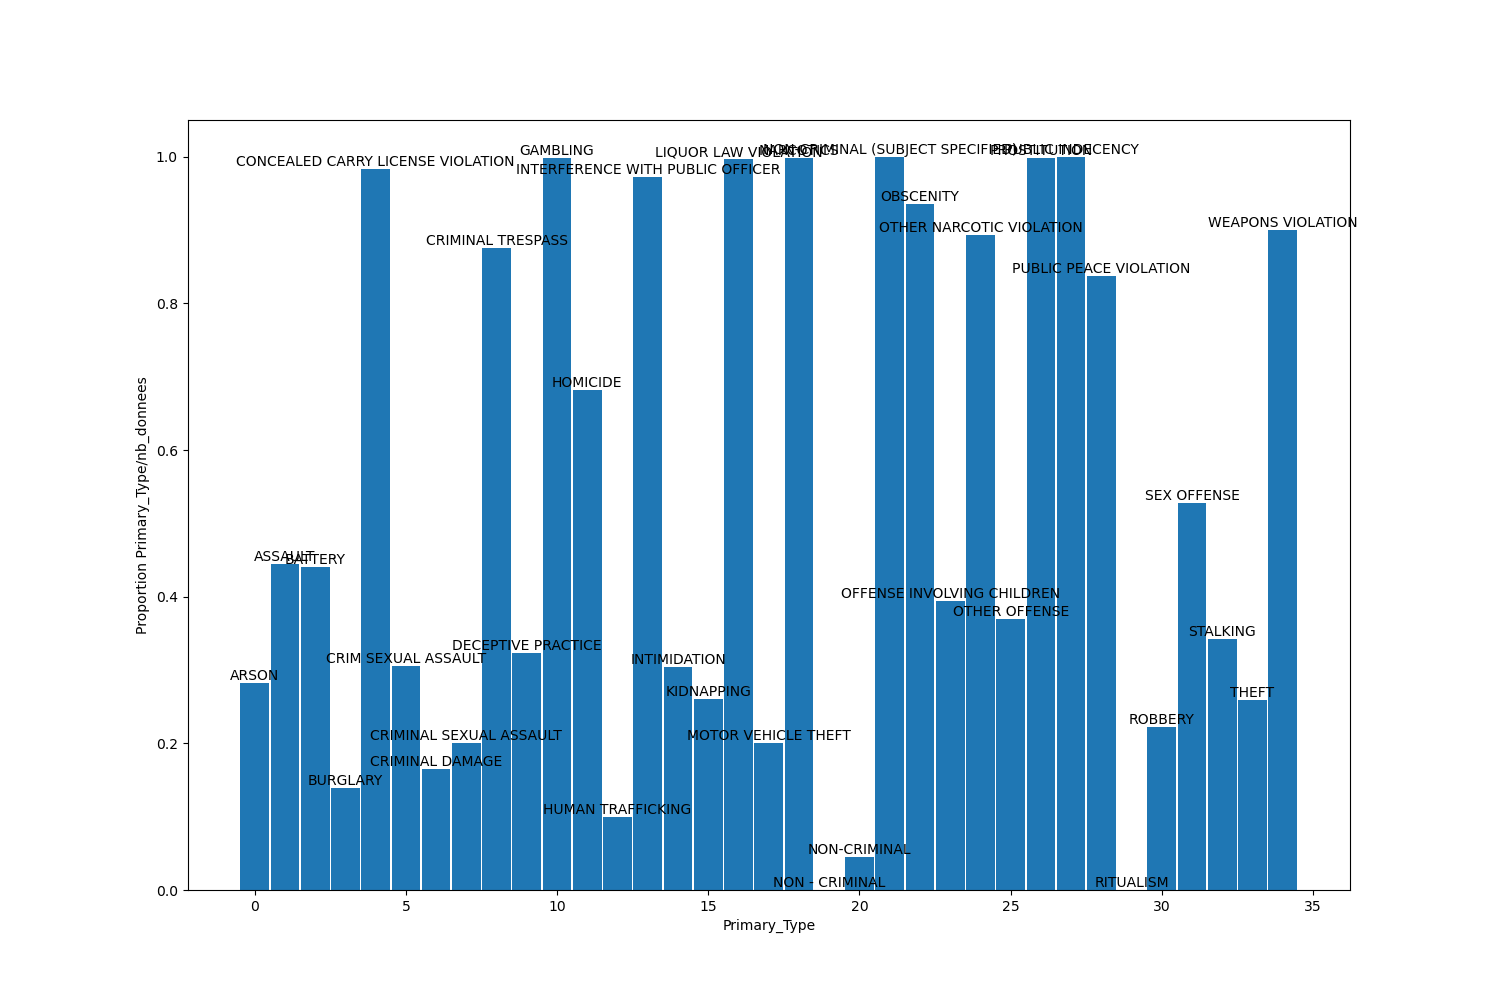
\includegraphics[scale=.2]{images/typeArrestation.png}
		    \caption{Types de crimes avec le plus d'arrestation}
		    \label{B}
	    \end{subfigure}
	    \caption{Aperçu }
    \end{figure}
    La Figure \ref{A} nous montre que les crimes les plus représentés sont les 
    agressions (\textit{battery}), le trafic de de drogue (\textit{narcotics}) 
    et les vols (\textit{threft}).

    \begin{wrapfigure}{r}{0.5\textwidth}
	    \centering
	    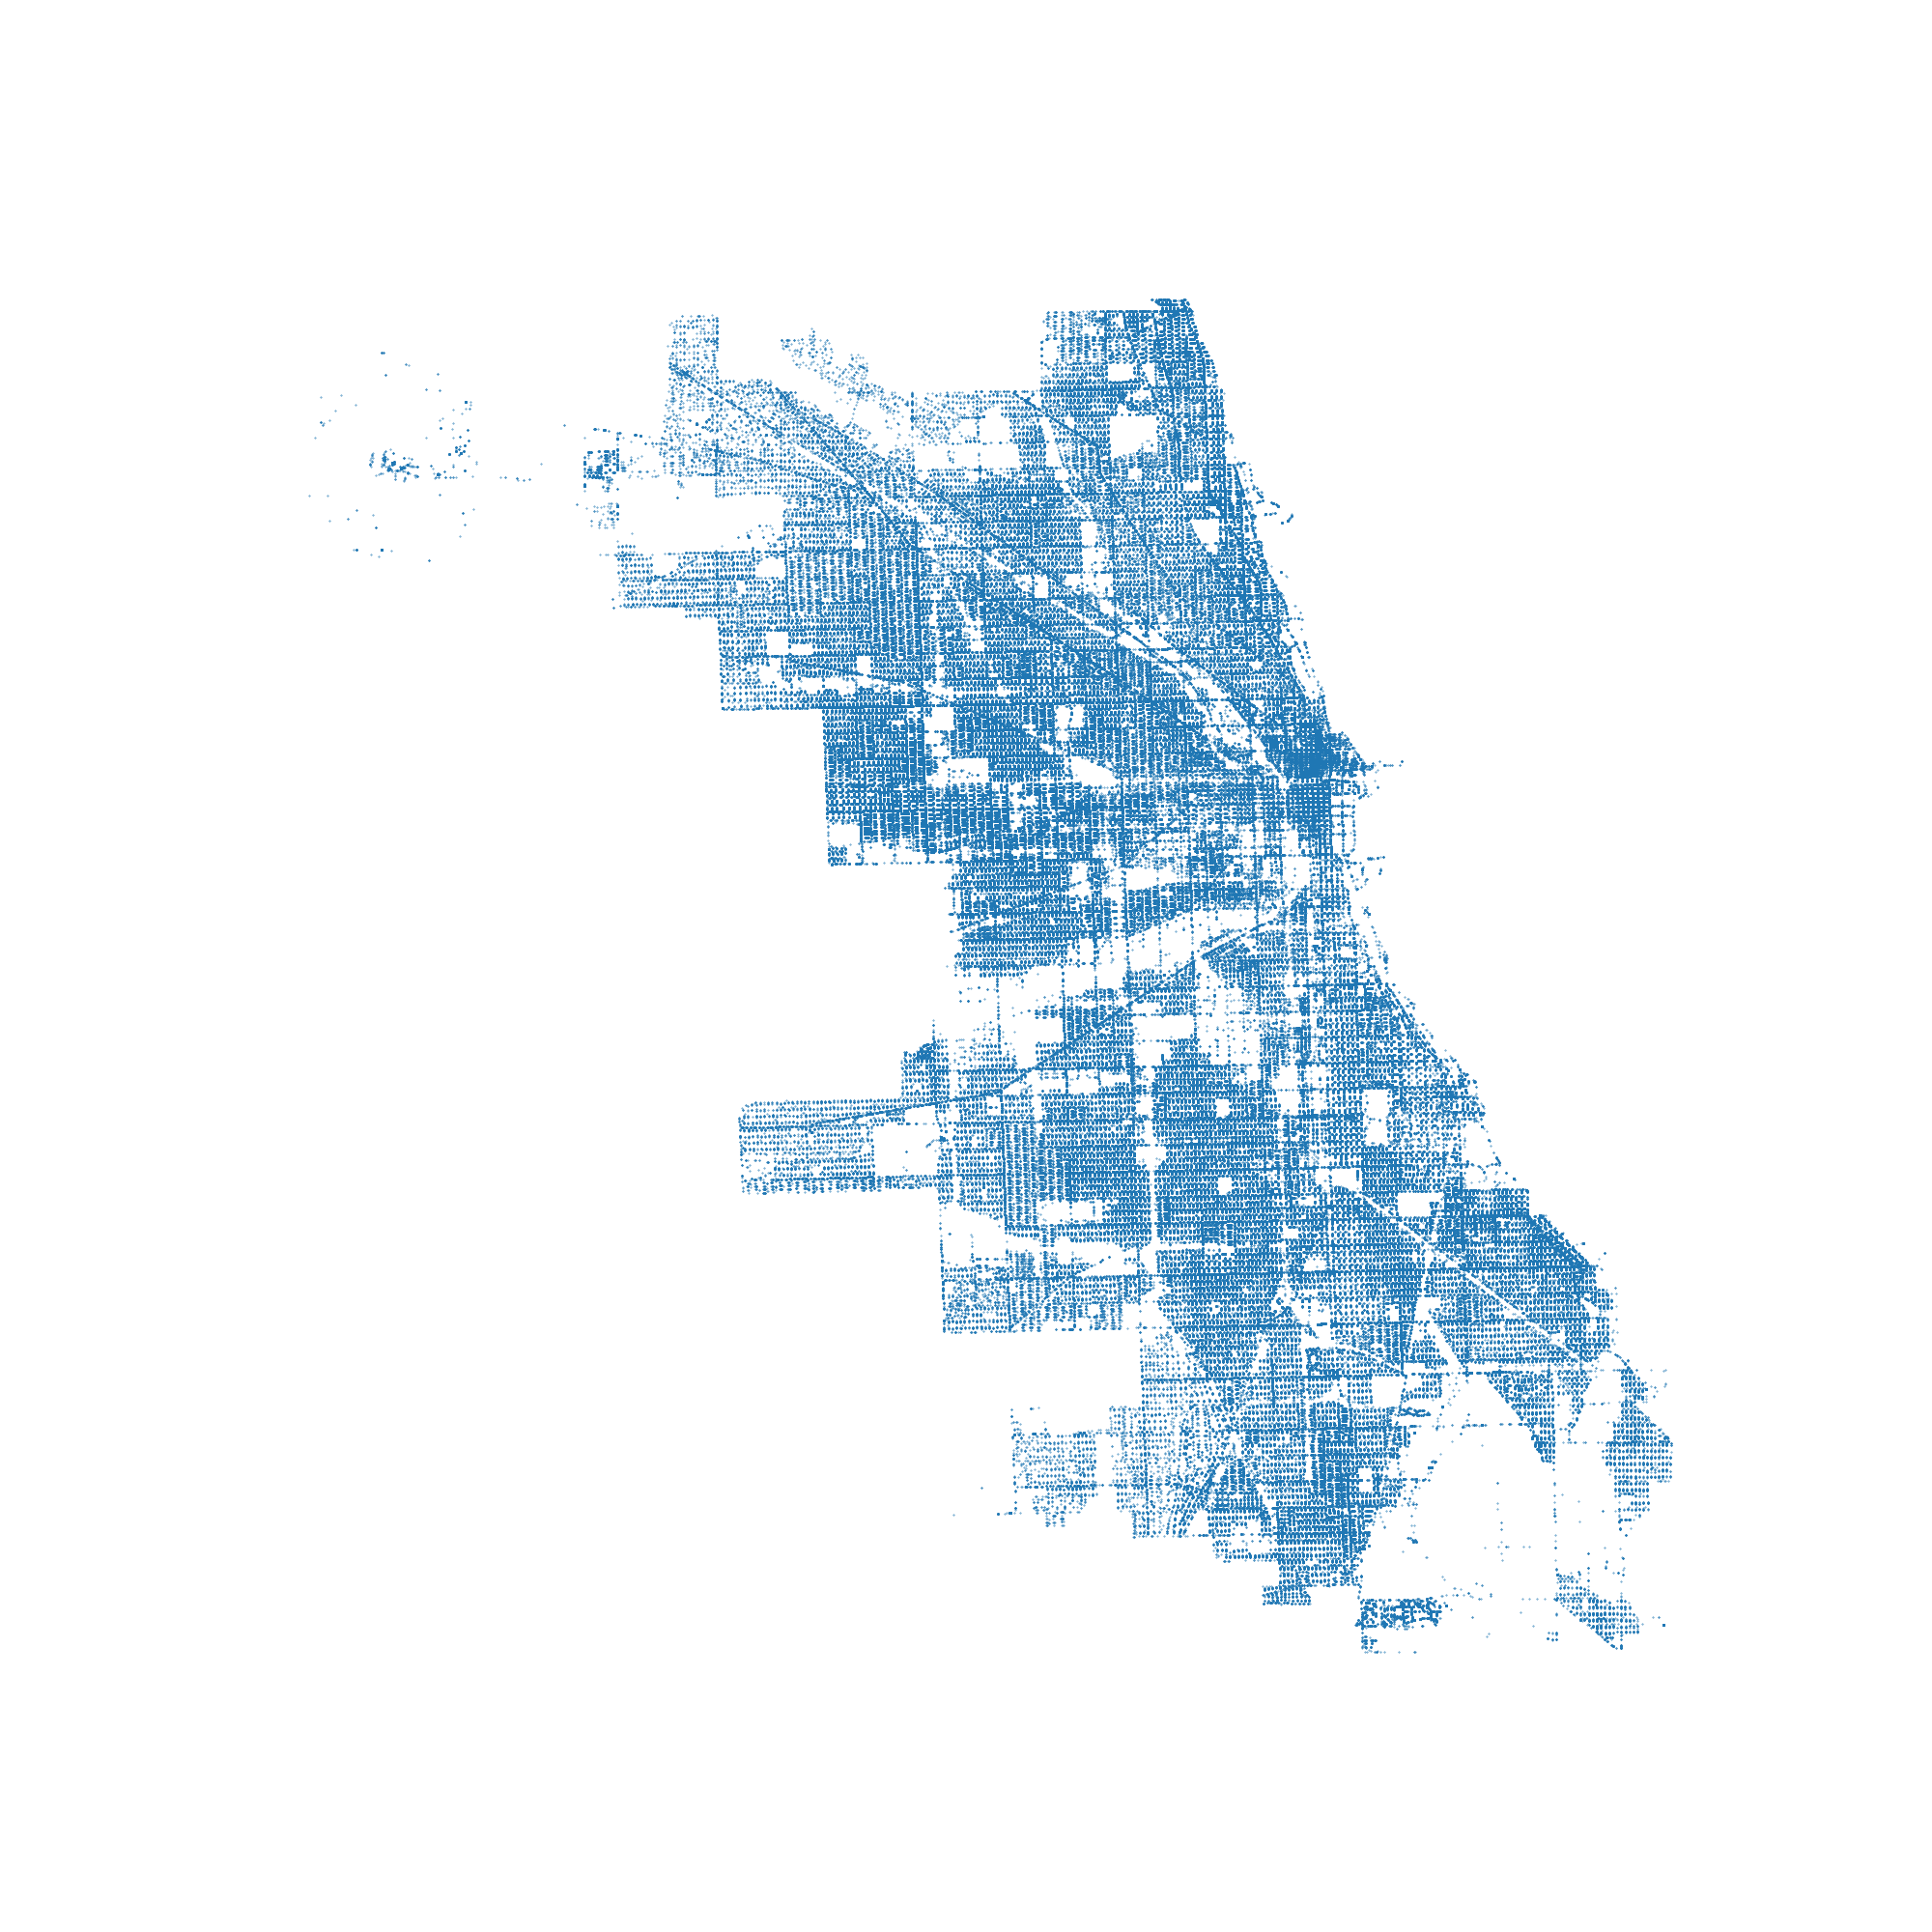
\includegraphics[width=0.5\textwidth]{images/carte_chicago.png}
	    \caption{Carte représentant l'ensemble des crimes commis à Chicago}
	    \label{C}
    \end{wrapfigure}

    D'après la Figure \ref{B}, on voit que certains crimes sont quasiment toujours suivis 
    d'une arrestation, c'est le cas des paris illégaux, du port d'armes dissimulées, 
    des crimes liés à l'alcool et l'obscénité.
    Cette même Figure nous apprend qu'il y a moins de 20\% d'arrestation pour les 
    cambriolages, le trafic d'humains, les braquages et les vols de véhicules motorisés.
    Enfin, on voit sur la Figure \ref{C} la carte de Chicago se dessiner, où chaque
    point représente un crime.

    \section{Définition du problème}
    Notre problème sera le suivant. Il s'agira de déterminer si il y aura
    oui ou non une arrestation à la suite d'un crime. 
    Pour être plus précis, étant donné le lieu, la description et la date du crime, 
    il faudra dire si cela va mener à l'arrestation d'un suspect.
    C'est une tâche de classification
    binaire, en apprentissage supervisé.

    \section{Préprocessing}
    Comme le dataset contenait peu de features, 
    nous avons effectué plusieurs modifications sur le dataset 
    avant d'entraîner notre modèle.
    De plus, certaines features étaient uniques pour chacun de nos crimes.

    On rappelle que notre dataset contient 7 millions d'entrées, on peut se permettre
    de faire quelques changements.
    Nous avons tout d'abord supprimé les données qui contenaient des features vides,
    et nous avons équilibré le dataset en mettant autant de crimes avec arrestation que de crimes sans arrestation.
    Cela a été fait avec des commandes shell pour la rapidité et la simplicité. 
    Voici les commandes effectuées.

    \begin{Verbatim}
    ## Nettoyer les données
    grep -v -E '(,0,0,2)|(,,)' Crimes2001.csv  > CrimesClean.csv
    
    ## Equilibrer les données
    # Ici on sépares à l'aide d'expressions régulières les arrested et les non arrested
    grep -E '^(([^,]*,)|("[^"]*",)){8}false' CrimesClean.csv > CrimesCleanNonArrested.csv
    grep -E '^(([^,]*,)|("[^"]*",)){8}true' CrimesClean.csv > CrimesCleanArrested.csv
 
    # Ici on recombine en n'oubliant pas le header contenant le nom des features
    head -n 1 CrimesClean.csv > CrimesEq.csv
    n=$(wc -l CrimesCleanArrested.csv | grep -E -o '[0-9]+ ')
    cp CrimesCleanArrested.csv tmp.csv
    shuf -n $n CrimesCleanNonArrested.csv >> tmp.csv
    shuf tmp.csv >> CrimesEq.csv
    \end{Verbatim}

    \begin{wrapfigure}{r}{0.5\textwidth}
	    \centering
	    \includegraphics[width=0.5\textwidth]{images/carte_densité.png}
	    \caption{Clusters des crimes de Chicago}
	    \label{E}
    \end{wrapfigure}
    Ici le fichier CrimesEq.csv contient 3,4 millions de crimes, on ne va pas travailler avec 
    autant de données et se limiter 1 million.
    L'étape suivante a été de supprimer les features uniques et celles qui se répétaient:
    \begin{itemize}
	    \item ID
	    \item Case Number
	    \item Block
	    \item Updated On
	    \item Longitude
	    \item Latitude
	    \item Location
    \end{itemize}
    À partir de la feature \textit{date}, nous avons extrait les features suivantes
    \begin{itemize}
	    \item Part of the day
	    \item Weekday
	    \item Weekend
	    \item Month
	    \item Hour
    \end{itemize}
    Enfin, à partir des coordonnées géographiques, nous avons appliqué un algorithme
    de k-moyennes pour séparer les zones de Chicago et en déduire une nouvelle
    feature \textit{Cluster}. 
    Voici ce que l'on obtient (Figure \ref{E}) lorsque l'on affiche la localisation des crimes en
    fonction de leurs clusters.
    Sur cette dernière carte, les clusters plus rouges concentrent le plus de crimes.

    \section{Choix d'algorithme}
    Comme notre dataset est assez conséquent, nous avons utilisé les algorithmes 
    de la bibliothèque \textit{scikit-learn}.
    Pour classifier nos crimes, nous utilisons le DecisionTree et le modèle Gaussien Naïf.
    Différentes fonctions dans le fichier main.py nous ont permis de déterminer
    les meilleurs hyper-paramètres à choisir pour le DecisionTree.
    \begin{figure}[H]
	    \centering
	    \begin{subfigure}{.45\textwidth}
		    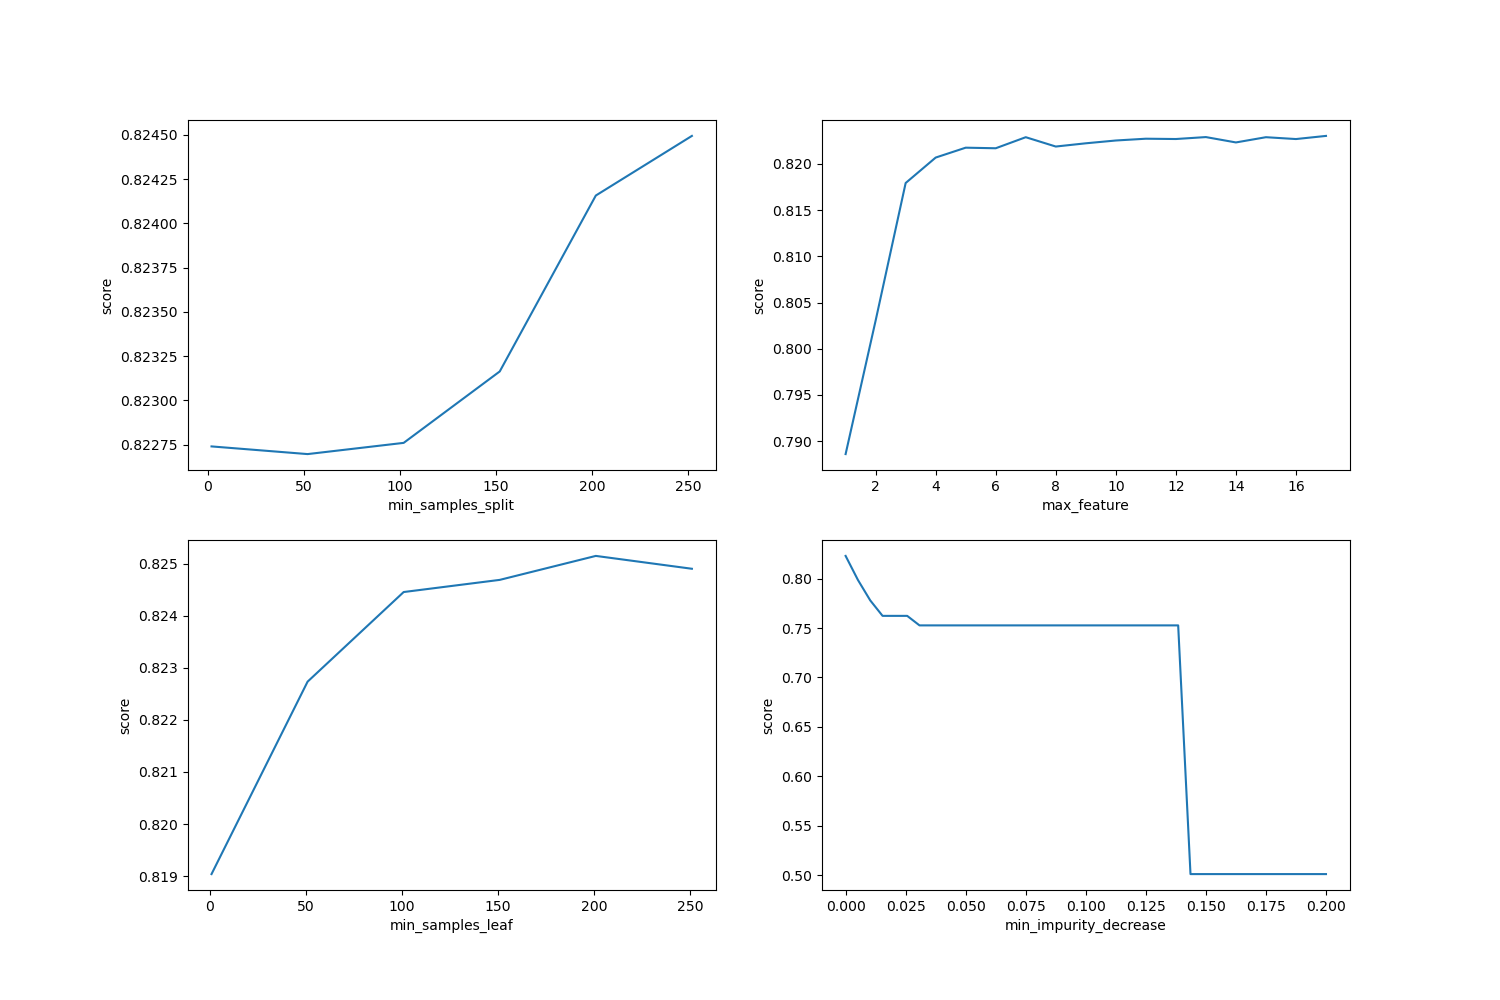
\includegraphics[scale=.2]{images/bestParamDecisionTree.png}
		    \caption{Cross-validation pour le DecisionTree}
	    \end{subfigure}
	    \begin{subfigure}{.45\textwidth}
		    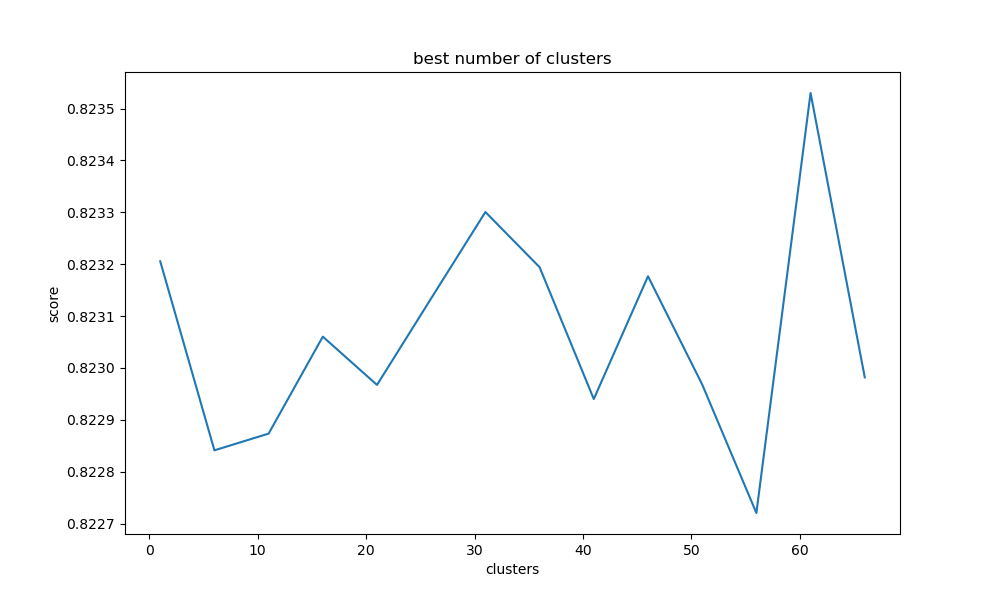
\includegraphics[scale=.3]{images/bestNumClusters.png}
		    \caption{Choix du meilleur nombre de clusters}
	    \end{subfigure}
    \end{figure}
    Les hyper-paramètres qui ont été testés sont le \textit{min\_sample\_split}, le \textit{min\_sample\_leaf},
    le \textit{max\_features}, le \textit{min\_impurity\_decrease}, le nombre de clusters et le 
    nombre de données.

    Nous avons également essayé d'utiliser un RandomForestClassifier. 
    Le score était substantiellement identique au DecsionTree, mais avec un 
    temps de calcul deux à trois fois supérieur. On pense que c'est du au
    fait que avons déjà beaucoup de données sur lesquelles nous entraîner, 
    et que le RandomForest serait plus adapté pour un dataset plus restreint.

    \section{Comparaison des modèles}

    L'arbre de décision est un algorithme de classification qui nous aide 
    à prendre des décisions:
    selon le type de crime, selon le lieu, le moment etc., y a-t-il eu 
    arrestation ou pas?  Pour chaque feature, il essaye de répondre à des  
    questions sur celles-ci afin de les séparer en différentes catégories:
    Le crime a-t-il eu lieu sur la place publique ou dans un appartement?
    (on peut voir sur la Figure \ref{D} que \textit{location description} est une feature
    importante à la décision, car la question posée sur cette feature est pertinente).
    L'arbre de décision que nous avons obtenu est vraiment grand, car beaucoup de
    features, mais nous avons créé un DecisionTree avec une partie restreinte de
    nos features afin de pouvoir le visualiser:

    \begin{figure}[H]
            \centering
	    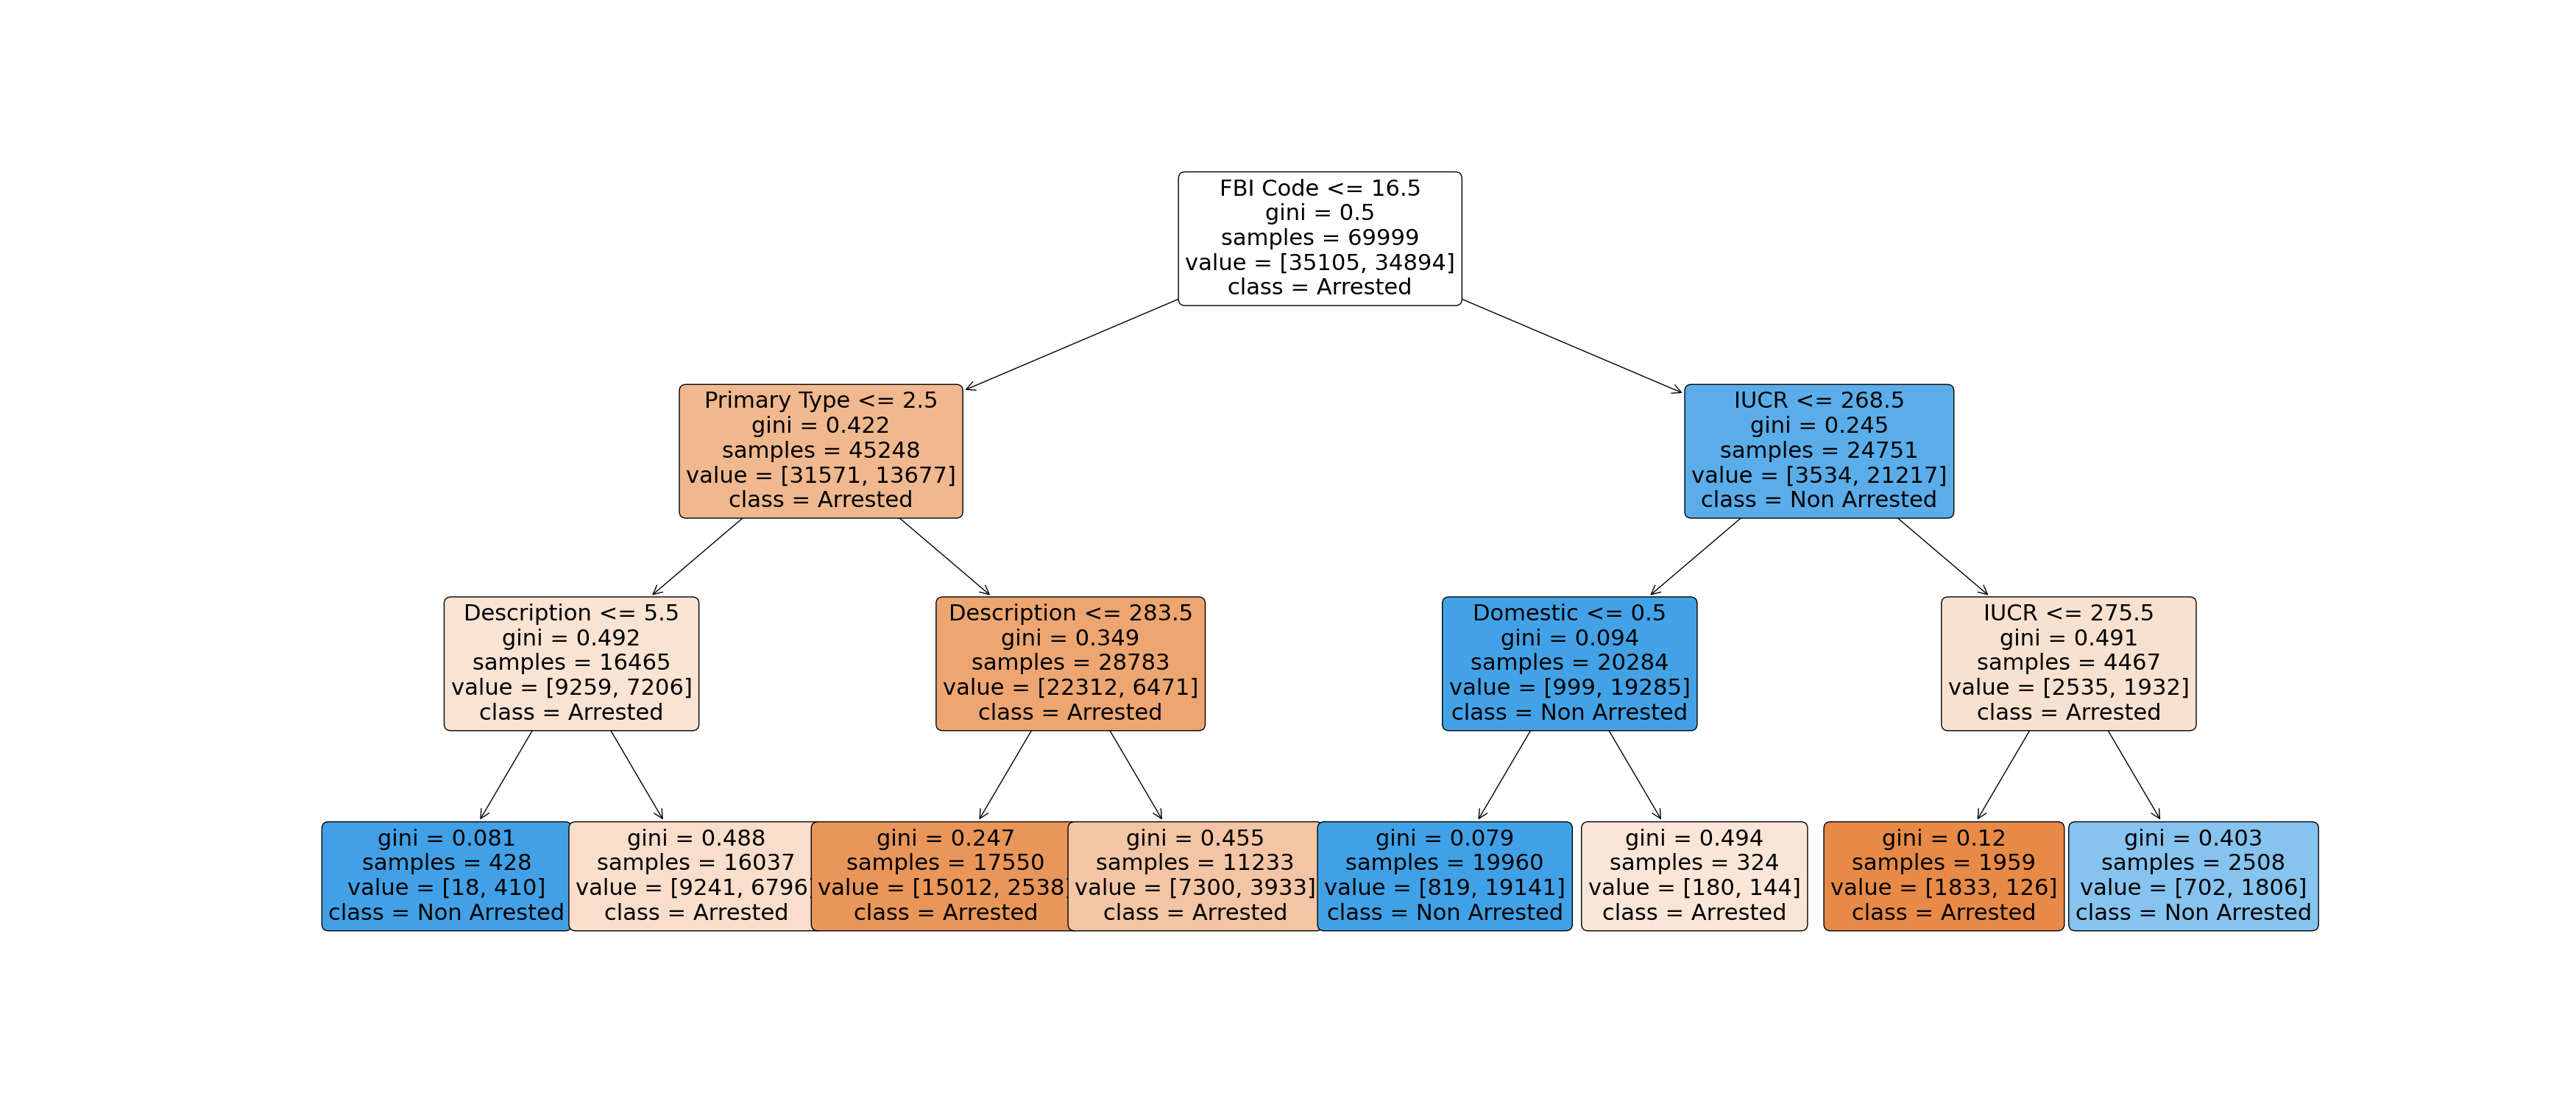
\includegraphics[scale=.18]{images/treeExample.png}
	    \caption{Exemple d'un DecistionTree}
    \end{figure}
    \begin{figure}[H]
            \centering
	    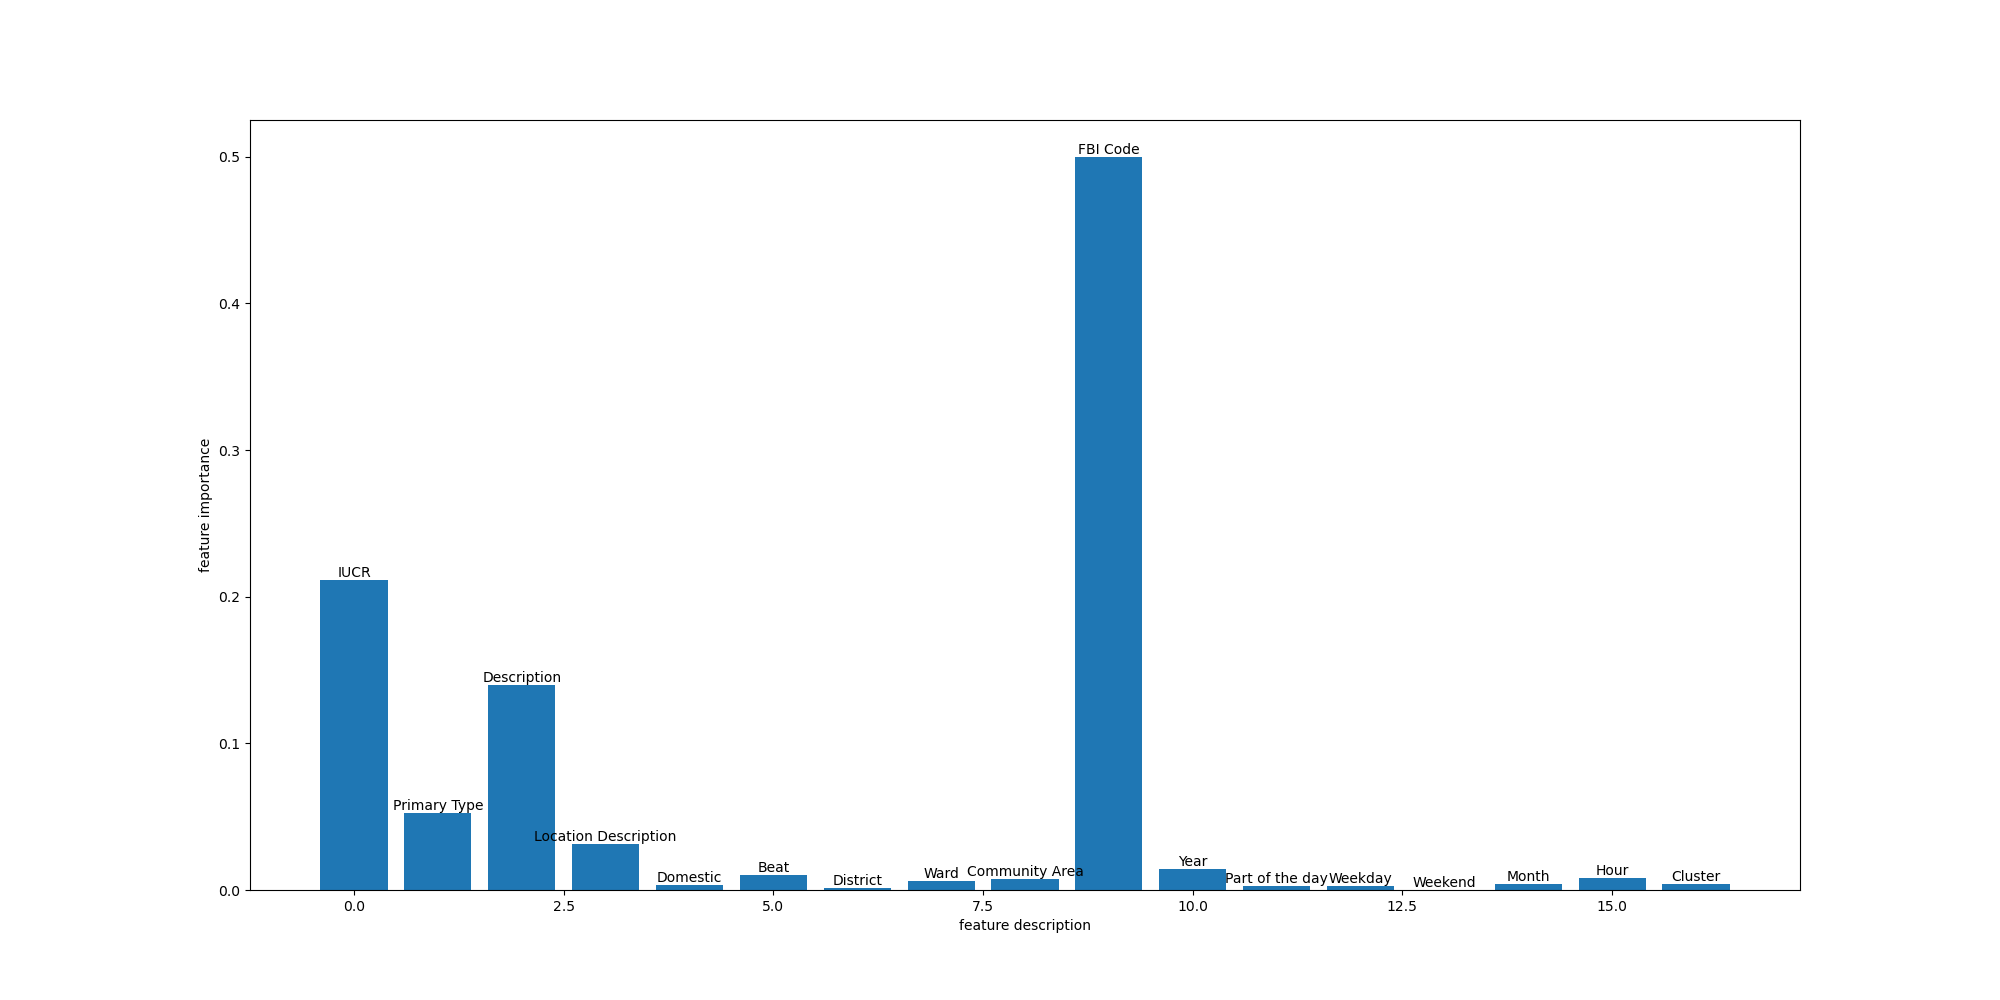
\includegraphics[scale=.3]{images/feature_importance.png}
	    \caption{Importance des features pour le DecisionTree}
	    \label{D}
    \end{figure}


    Le modèle bayésien naïf est un modèle basé sur l'EMV
    (Estimateur du Maximum de Vraisemblance).
    Le but est simple, maximiser la vraisemblance. 
    Cependant une hypothèse importante de ce modèle est l'indépendance de chaque donnée,
    ce que l'on ne peut pas garantir dans le cadre de notre projet.
    Ainsi, on peut prévoir une score moyen pour ce modèle avec nos données.

    Comme nous avons beaucoup de données (1M pour les calculs des scores),
    le bayésien naïf va avoir du mal, alors que cela ne change pas grand
    chose pour le DecisionTree.

    \section{Présentation des résultats}

    \begin{figure}[H]
	    \begin{subfigure}{.45\textwidth}
		    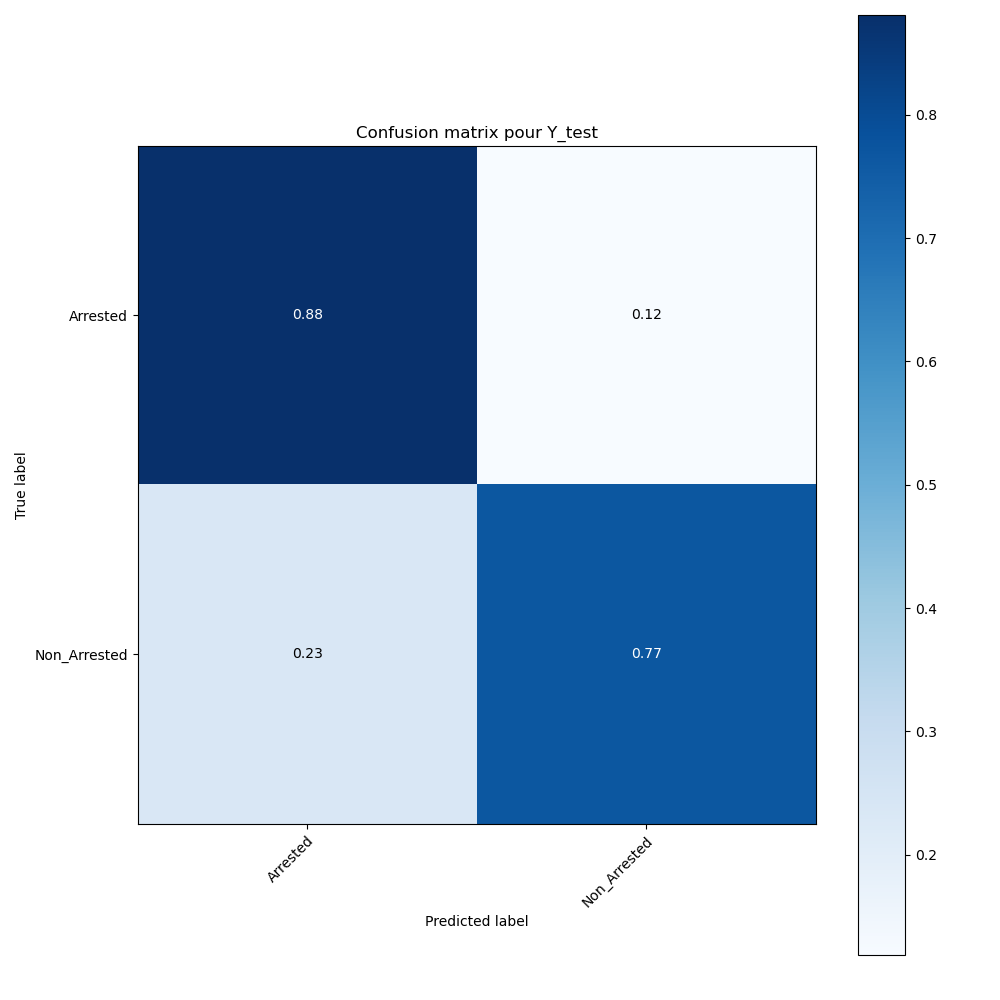
\includegraphics[scale=.314]{images/MatriceConfusionDecisionTree.png}
		    \centering
		    \caption{Matrice de confusion du DecisionTree}
	    \end{subfigure}
	    \begin{subfigure}{.45\textwidth}
		    \centering
		    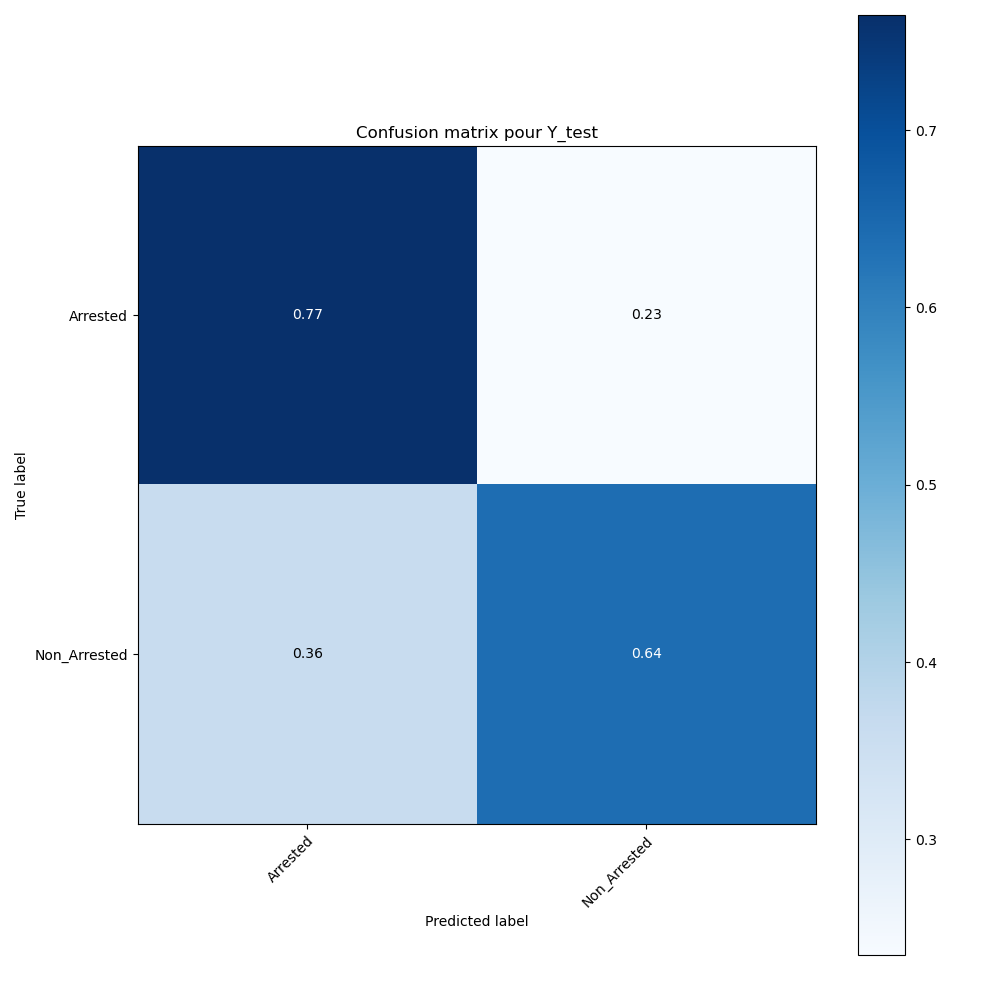
\includegraphics[scale=.35]{images/MatriceConfusionGauss.png}
		    \caption{Matrice de confusion du Bayésien Naïf}
	    \end{subfigure}
    \end{figure}

    Voici les matrices de confusion générées pour le DecisionTree et le modèle 
    Bayésien Naïf, entrainés sur nos 1 millions de données. 
    On peut voir que ces deux modèles arrivent 
    mieux à valider le fait qu'il y ait arrestation que le fait qu'il n'y ait 
    pas d'arrestation.

    Après optimisation des paramètres, les scores obtenus pour nos deux modèles sont:
    \begin{Verbatim}
    Score GaussNB :  0.703753
    Score DecisionTree :  0.82345
    \end{Verbatim}

    La comparaison des modèles nous a donné raison, l'arbre de décision nous donne
    un meilleur score que le bayésien naïf.

    Voici quelques exemples concrets de nos prédictions, sur l'ensemble de test.
    \begin{figure}[H]
	    \centering
	    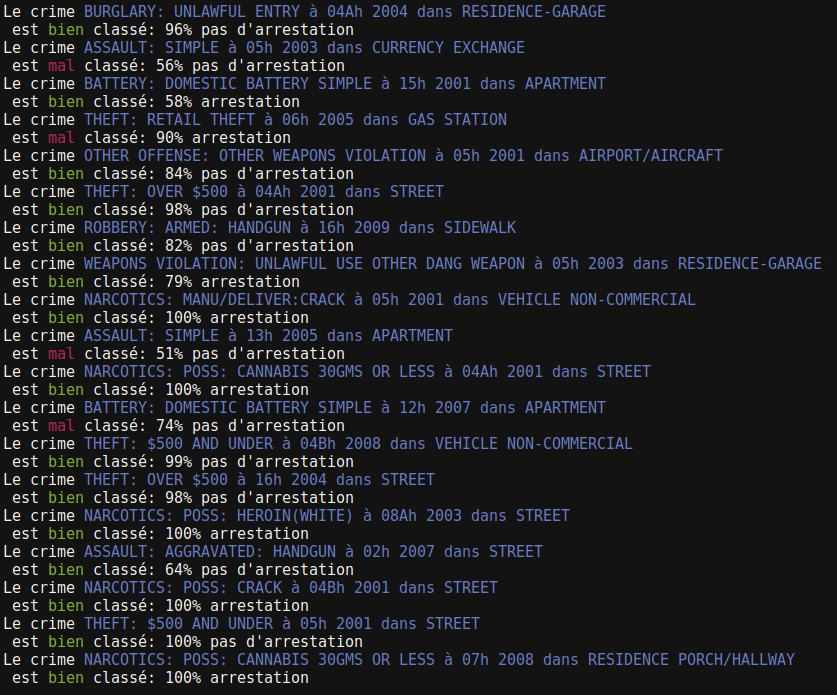
\includegraphics[scale=.4]{images/results.png}
	    \caption{Exemples de prédictions avec les pourcentages}
    \end{figure}


    \section{Conclusion}
    Dans ce projet, nous avons pu comparer différents modèles de
    classification. 
    Ce qui nous a particulièrement plu, c'était de travailler sur le dataset
    avant d'entraîner le modèle. En effet, nos données contenaient peu de
    features et n'étaient pas très bien équilibrée.
    Néanmoins, nous obtenons un score très correct, nous pouvons prédire à
    plus de 80\% si pour un crime donné, il y aura une arrestation ou non.

    Pour aller plus loin, il aurait été intéressant d'ajouter des features
    externes au dataset, telles que des données météorologiques, des
    évènements sociaux ou politique. Cela nous aurait demandé de créer un
    nouveau dataset, mais il aurait été très intéressant de voir à quel 
    point on peut augmenter notre score de cette manière.

    Enfin, notre modèle a quelques limites. Tous les crimes du dataset sont
    relevés par la police de Chicago. Donc certains de ces crimes sont
    forcements suivis d'une arrestation. C'est par exemple le cas de la
    détention de drogue, qui est un crime flagrant.
    De plus, on peut facilement imaginer que l'ensemble des crimes commis
    dans la ville ne sont pas répertoriés. Le dataset est donc biaisé sur ce
    point.

\end{document}
